%!TEX root = ../TAMUTemplate.tex
%%%%%%%%%%%%%%%%%%%%%%%%%%%%%%%%%%%%%%%%%%%%%%%%%%%
%
%  New template code for TAMU Theses and Dissertations starting Fall 2016.
%
%  Author: Sean Zachary Roberson
%    Version 3.16.09
%  Last updated 9/12/2016
%
%%%%%%%%%%%%%%%%%%%%%%%%%%%%%%%%%%%%%%%%%%%%%%%%%%%

%%%%%%%%%%%%%%%%%%%%%%%%%%%%%%%%%%%%%%%%%%%%%%%%%%%%%%%%%%%%%%%%%%%%%%%
%%%                           SECTION II
%%%%%%%%%%%%%%%%%%%%%%%%%%%%%%%%%%%%%%%%%%%%%%%%%%%%%%%%%%%%%%%%%%%%%%

\chapter{\uppercase {Theoretical Framework}}
\label{ch:theoretical_framework}

Since the mid-1970s, the Standard Model (SM) of particle physics has been the leading theory describing three of the four known fundamental forces (not including gravity) as well as classifying all of the known elementary particles.
Even during it's formative years, the SM's success at predicting new particles (i.e. the top quark in 1995) and describing the properties of known particles (i.e. $W^{\pm}$ to $Z^{0}$ mass ratio) was undeniable.
The model's roots can be traced back to 1930 when Herman Weyl was able to describe electromagnetism as a local symmetry represented by the Lie group $U\left(1\right)$~\cite{Weyl1929}.
In 1954 Yang and Mills created a theory which tried to extend the idea of gauge theory to non-abelian groups~\cite{PhysRev.96.191}.
This laid the ground work for Sheldon Glashow to combine the electromagnetic and weak interactions in 1961~\cite{GLASHOW1961579}.
This combined interaction is described by the $SU\left(2\right){\times}U\left(1\right)$ group.
In 1967 Steven Weinberg and Abdus Salam~\cite{PhysRevLett.19.1264,salam1968} continued this work by adding in the Higgs mechanism first proposed by Robert Brout and Francois Englert~\cite{PhysRevLett.13.321}, Peter Higgs~\cite{PhysRevLett.13.508,Higgs:1966ev}, and Gerald Guralnik, Carl. R. Hagen, and Tom Kibble~\cite{PhysRevLett.13.585,Kibble:1967sv}.
Although all of these theorist contributed to this advancement, the mechanism eventually became known as the Brout-Englert-Higgs (BEH) mechanism.
The model entered its current form around 1964 with the introduction of the strong force and quantum chromodynamics (QCD)~\cite{Neeman:1961jhl,GellMann:1962xb,GellMann:1964nj,Zweig:1981pd,Fritzsch:1972jv}.
The initial theory by Gell-Man and Zweig only included the up, down, and strange quarks and was incomplete until the introduction of the color charge by Greenberg~\cite{PhysRevLett.13.598}.
The full theory is described by the symmetry group
\begin{equation}\label{eq:standard_model_symmetry_group}
SU\left(3\right)_{C}{\otimes}SU\left(2\right)_{L}{\otimes}U\left(1\right)_{Y}
\end{equation}
where $SU\left(2\right)_{L}{\otimes}U\left(1\right)_{Y}$ is the electroweak (EW) symmetry group describing both the electromagnetic and weak interactions and $SU\left(3\right)_{C}$ is the symmetry group describing the strong interaction~\cite{Burgess2007,Aitchison2012}.

The rest of this chapter will discuss the standard model, both its structure and some of its mathematical underpinnings, in more detail.
Section~\ref{sec:standard_model} will introduce the particle content of the SM.
The QFTs that govern the SM interactions will be discussed in sections~\ref{sec:QED} to~\ref{sec:higgs_mechanism}.
In section~\ref{sec:BSM} we will briefly reference how Higgs physics can relate to physics beyond the SM.
More information about the history of the standard model can be found in appendix~\ref{appendix:standard_model_history}.

\section{The Standard Model}
\label{sec:standard_model}

The standard model is a locally gauge-invariant quantum field theory (QFT) in four-dimensional Minkowski space~\cite{Burgess2007,Barnes2010}.
The structure and particle content of the SM can be found in fig~\ref{fig:standard_model}.
The SM is composed of 12 fermions, the particles that make up matter, and 4 gauge bosons, the force-carrying particles which mediate the electromagnetic, weak, and strong interactions.
On its own, the basic symmetries of the standard model require that the gauge bosons (W$^\pm$,Z,$\gamma$,gluons) be massless.
However, we know that this is not true as experiments have shown that the $W$ and $Z$ bosons have quite a large mass.
The aforementioned Higgs mechanism takes care of this by spontaneously breaking the electroweak symmetry, giving mass to the quarks, the leptons, and the $W$ and $Z$ bosons~\cite{PhysRevLett.19.1264,salam1968,Dawson:1998yi}.

\begin{figure}[!hbt]
	%\scalebox{.45}{\input{StandardModel}}
	\centering
	\resizebox{0.95\textwidth}{!}{\input{StandardModel_CERNWebfest2012}}
	\caption{The Standard Model of particle physics. The model includes three generations of matter particles (leptons and quarks) as well as the gauge and Higgs bosons. Included in this drawing are the particle names, symbols, masses, spin, electric charge, and color charge, if applicable.}
	\label{fig:standard_model}
\end{figure}

Fermions are particles which obey Fermi-Dirac statistics and the Pauli exclusion principle, meaning that no two fermions may occupy the same quantum state within a given quantum system.
These particles have half-integer spin, often denoted as spin-1/2 particles, which means that their intrinsic angular momentum is $\hbar/2$.
For every fermion $f$ in the SM there exists an anti-fermion $\bar{f}$, which has an identical mass, but opposite quantum numbers.
The fermions in the SM are separated into six leptons and six quarks with these further separated into 3 generations of pairs of particles.
Each subsequent generation is ostensibly a heavier version of the previous generation, with the same quantum numbers.\footnote{The neutrinos may have a different mass ordering.}

Each generation of lepton can be broken down into a charged and neutral lepton.
For instance, the first generation is composed of the electron (\Pe), with charge $-\Pe$, and the electron neutrino ($\Pgn_{e}$).
The second and third generations contain the muon (\Pmu) and tau (\Ptau) along with their associated neutrinos.
Although the SM specifies that the neutrinos are massless, experiments have shown that this is not true.
While their exact masses are still unknown, upper bounds have been places on these and can be seen in fig~\ref{fig:standard_model}.
Each generation of lepton has an associated quantum number, called the lepton number, defined as $L_{\ell}=n_{\ell}-n_{\bar{\ell}}$.
First generation leptons have quantum numbers $L_{e}=+1$ and $L_{\mu}=L_{\tau}=0$ while the second and third generations have value $+1$ for their associated lepton number and zero otherwise.
The antileptons have oppositely signed lepton numbers.
The lepton numbers are a conserved quantity in the SM, which means that only lepton-antilepton pairs can be created or destroyed.\
That being said, neutrino oscillations, the phenomena of neutrinos changing flavor from one generation to the next, has been observed~\cite{Maltoni:2004ei}.
While this violates the conservation of lepton numbers within a generation, the total lepton number $L{\equiv}L_{e}+L_{\mu}+L_{\tau}$ may still be conserved.
All leptons interact through the weak interaction, but only the charged leptons interact using the electromagnetic interaction.
Because leptons lack the color charge they do not interact using the strong force.

Like the leptons, the three generation of quarks can be broken into one up-type quark and one down-type quark, categories which gain their name through the content of the first generation containing the up (\cPqu) and down (\cPqd) quarks.
The second generation is made up of the charm (\cPqc) and strange (\cPqs) quarks while the third is made up of the top (\cPqt) and bottom (\cPqb) quarks.
The up-type quarks have fractional electric charge of $Q=+2e/3$ and the bottom-type quarks have electric charge $Q=-e/3$.
As in the case of the leptons, the quarks have an associated baryon quantum number, $B$.
This quantity is conserved in all SM interactions and no exception has every been seen.
This means that only quark-antiquark pairs may be created or destroyed and also results in the stability of the lightest baryon, the proton.
Baryon number is defined as $B=\frac{1}{3}\left(n_{q}-n_{\bar{q}}\right)$, where, for example, the baryon number for a quark is $+1/3$ and $-1/3$ for an antiquark.
Quarks may interact through the electromagnetic and weak interactions, but unlike the lepton, quarks can also interact via the strong force.
This is because quarks also have color charge, which can have three values referred to as red, green, or blue. 
Antiquarks may contain charges of anti-red, anti-green, or anti-blue.
In the SM colorless particles are forbidden from existing on their own, which means that individual quarks, often refered to as bare quarks, have never been seen in nature.
Instead, quarks are always found as constituents of bound states called hadrons.
This group of composite particles may be further divided into mesons, bound states of a quark-antiquark pair, and baryons, bound states of three quarks and antiquarks.
The hadrons contain quark and antiquark combinations such that the bound state is a color singlet, often referred to as being colorless.
Mesons contain color-anticolor pairs while baryons consist of red, green, and blue charged quarks.
The masses of the quarks are hard to measure due to their confinement in hadrons, however, global averages have been made.

\section{Quantum Electrodynamics \& the Electromagnetic Interaction}
\label{sec:QED}

Quantum electrodynamic (QED) is a quantum field theory which describes the dynamics of the electromagnetic interaction and corresponds to the $U_{EM}\left(1\right)$ group.
In a QFT, particles are represented by fields, which are in turn represented mathematically by Lagrangian densities $\mathcal{L}$.
QED was formulated to described the interactions of spin-1/2 particles, namely leptons and quarks.
Like a classical field theory, the dynamics of a quantum system are described by a Lagrangian.
QED is described by the Dirac Lagrangian density
\begin{equation}\label{eq:dirac_lagrangian_density}
\mathcal{L}=i\bar{\psi}\gamma^{\mu}\partial_{\mu}\psi-m\bar{\psi}\psi
\end{equation}
where $\psi$ a four-component column vector representing the wave function of a spin-1/2 particle\footnote{$\psi$ is a field known as a Dirac spinor.}, $\gamma^{\mu}$ are the four Dirac gamma matrices, $\bar{\psi}\equiv\psi^{\dagger}\gamma^{0}$, and $m$ is the mass of the particle.

In order for QED to be gauge invariant it must be invariant under both local and global gauge transformations.
Let there exist a global $U\left(1\right)$ transformation
\begin{equation}\label{eq:global_u1_transformation}
	\psi\rightarrow\psi'=e^{-i\alpha}\psi
\end{equation}
with constant $\alpha$.
Then $\psi$ in the Lagrangian~\ref{eq:dirac_lagrangian_density} can be replaced by equation~\ref{eq:global_u1_transformation}, which means that $\mathcal{L}\rightarrow\mathcal{L}'=\mathcal{L}$.
Therefore QED is invariant under this type of transformation.
If instead we have $\alpha\rightarrow\alpha\left(x\right)$ where $\alpha$ is allowed to vary as a function of spacetime, then equation~\ref{eq:global_u1_transformation} becomes a local $U\left(1\right)$ transformation.
In this case equation~\ref{eq:dirac_lagrangian_density} becomes
\begin{equation}\label{eq:local_transformation}
	\mathcal{L}\rightarrow\mathcal{L}'=\mathcal{L}+\bar{\psi}\gamma^{\mu}\left(\partial_{\mu}\alpha\left(x\right)\right)\psi
\end{equation}
and is thus not invariant under the local transformation as is.
To return the gauge invariance we can replace the partial derivative in the Lagrangian density by a covariant derivative
\begin{equation}\label{eq:covariant_derivative}
	D_{\mu}=\partial_{\mu}+iqA_{\mu}
\end{equation}
, where $q=-e$ is the electron charge, in case of an electron, and $A_{\mu}$ is a new gauge field representing the photon, the mediator of electromagnetic interactions.
This new gauge field transforms as
\begin{equation}\label{eq:photon_transformation}
	A_{\mu}{\rightarrow}A_{\mu}'=A_{\mu}+\partial_{\mu}\chi\left(x\right)
\end{equation}
, where $\chi\left(x\right)$ is an arbitrary function of spacetime.
When the transformation in equation~\ref{eq:global_u1_transformation} is made to a lepton field, the photon field transforms as in equation~\ref{eq:photon_transformation}, and $\chi\left(x\right)=\alpha\left(x\right)/q$, the covariant derivative transforms in the same way as $\psi\left(x\right)$, namely $D_{\mu}\psi\rightarrow\left(D_{\mu}\psi\right)'=e^{-i\alpha}D_{\mu}\psi$.
After the changes listed above, equation~\ref{eq:dirac_lagrangian_density} will take the locally gauge invariant form
\begin{equation}\label{eq:dirac_lagrangian_density_local_invariant}
	\mathcal{L}=\bar{\psi}\left(i\gamma^{\mu}D_{\mu}-m\right)\psi-\frac{1}{4}F^{\mu\nu}F_{\mu\nu}
\end{equation}
where
\begin{equation}\label{eq:electromagnetic_field_strength_tensor}
	F^{\mu\nu}=\left(\partial^{\mu}A^{\nu}-\partial^{\nu}A^{\mu}\right)
\end{equation}
is the electromagnetic field strength tensor.

Notice that in equation~\ref{eq:dirac_lagrangian_density_local_invariant} does not contain a $m^{2}A_{\mu}A^{\mu}$ term, which would be the mass of the gauge field.
This fits with experimental observations given that the photon is massless and thus the electromagnetic interaction has an infinite range.
Lagrangian~\ref{eq:dirac_lagrangian_density_local_invariant} does introduce lepton-photon interactions and does contain an $\ell^{+}\ell^{-}\gamma$ interaction and a term quadratic in the field strength tensor, which is the photon kinetic energy.
The complete QED Lagrangian can be created by generalizing to all leptons by $\psi\rightarrow\psi_{i}$ and summing over all leptons $i=e,\mu,\tau,u,d,c,s,t,b$ as in equation~\ref{eq:qed_lagrangian}.
\begin{equation}\label{eq:qed_lagrangian}
	\mathcal{L}=\sum_{i}\left[\bar{\psi}_{i}\left(i\gamma^{\mu}D_{\mu}-m_{i}\right)\psi_{i}\right]-\frac{1}{4}F_{\mu\nu}F^{\mu\nu}
\end{equation}

\section{Electroweak Interaction}
\label{sec:electroweak_interaction}

As mentioned in sec~\ref{ch:theoretical_framework}, the electromagnetic and weak interactions can be unified into a single, non-abelian gauge theory, work started by Yang \& Mills and then completed by Glashow, Weinberg, and Salam~\cite{Dawson:1998yi}.
In order to explain this unification, we will first work with a fermionic doublet representing and $SU\left(2\right)$ symmetry.
A doublet of Dirac fields can be represented as
\begin{equation}\label{eq:dirac_field_doublet}
	\psi=\doublet[r]{\psi_{1}\left(x\right)}{\psi_{2}\left(x\right)}
\end{equation}
The doublet will transform under the three dimensional rotation
\begin{equation}\label{eq:three_dimensional_rotation}
	\psi\rightarrow\exp\left<i\alpha^{i}\frac{\sigma_{i}}{2}\right>\psi
\end{equation}
This is again a global transformation, but note that by generalizing to higher order interaction we must use matrices instead of a local $\alpha\left(x\right)$ function to describe dynamics.
These matrices, $\sigma^{i}$, are the Pauli sigma matrices shown in equation~\ref{eq:pauli_sigma_matrices} and satisfy the identity $\sigma^{i}\sigma^{j}=\delta^{ij}+i\epsilon^{ijk}\sigma^{k}$ where $\epsilon^{ijk}=+1$ and where $\epsilon$ is an antisymmetric tensor.
\begin{equation}\label{eq:pauli_sigma_matrices}
	\sigma^{1}=\twoByTwo{0}{1}{1}{0},\text{ }\sigma^{2}=\twoByTwo{0}{-i}{i}{0},\text{ }\sigma^{3}=\twoByTwo{1}{0}{0}{-1}
\end{equation}

As in sec~\ref{sec:QED} we can turn equation~\ref{eq:three_dimensional_rotation} into a local transformation by having $\alpha\rightarrow\alpha^{i}\left(x\right)$ and thus
\begin{equation}
	\psi\left(x\right){\rightarrow}V\left(x\right)\psi\left(x\right)\text{, where }V\left(x\right)=\exp\left(i\alpha^{i}\left(x\right)\frac{\sigma^{i}}{2}\right)
\end{equation}
Still, the Lagrangian must be invariant under this transformation and in order to do this we introduce three vector fields $A_{\mu}^{i}\left(x\right)$, where $i=1,\;2,\;3$.
We once again use a covariant derivative
\begin{equation}
	D_{\mu}=\partial_{\mu}-igA_{\mu}^{i}\frac{\sigma^{i}}{2}
\end{equation}
, which means that the newly introduced fields transform as
\begin{equation}
	A_{\mu}^{i}\left(x\right)\frac{\sigma^{i}}{2}{\rightarrow}V\left(x\right)\left(A_{\mu}^{i}\left(x\right)\frac{\sigma^{i}}{2}+\frac{i}{g}\partial_{\mu}\right)V^{\dagger}\left(x\right)
\end{equation}
Unfortunately, this transformation is not trivial to calculate given that the Pauli matrices do not commute.
By assuming infinitesimally small transformations and expanding $V\left(x\right)$ to first order in $\alpha$ we obtain the simpler form
\begin{equation}
A_{\mu}^{i}\frac{\sigma^{i}}{2}{\rightarrow}A_{\mu}^{i}\frac{\sigma^{i}}{2}+\frac{1}{g}\left(\partial_{\mu}\alpha^{i}\right)\frac{\sigma^{i}}{2}+i\left[\alpha^{i}\frac{\sigma^{i}}{2},A_{\mu}^{i}\frac{\sigma^{i}}{2}\right]+...
\end{equation}
With the above ingredients the covariant derivative will transform as
\begin{equation}
	D_{\mu}\psi{\rightarrow}\left(1+i\alpha^{i}\frac{\sigma^{i}}{2}\right)D_{\mu}\psi
\end{equation}
and the field strength tensor will be
\begin{equation}
	F_{\mu\nu}^{i}=\partial_{\mu}A_{\nu}^{i}-\partial_{\nu}A_{\mu}^{i}+g\epsilon^{ijk}A_{\mu}^{j}A_{\nu}^{k}
\end{equation}
Given all of the above, the Yang-Mills Lagrangian will be
\begin{equation}\label{eq:yang_mills_lagrangian}
	\mathcal{L}=-\frac{1}{4}\left(F_{\mu\nu}^{i}\right)^{2}+\bar{\psi}\left(i\gamma^{\mu}\partial_{\mu}-igA_{\mu}^{i}\frac{\sigma^{i}}{2}\right)\psi
\end{equation}

Given the above process from Yang-Mills theory, we can now show how to obtain the electroweak interaction, which is based on a local $SU\left(2\right)_{L}{\times}U\left(1\right)_{Y}$ gauge symmetry. 
This process will follow what was done in section~\ref{sec:QED} in that requiring a local invariance will lead to the introduction of new gauge fields and determine their interactions.
It is also important to note that SM fermions can be grouped based on their chirality, which is a fundamental property of a particle and describes how the particles wave function will behave under rotation.
Spin-1/2 particles will pick up a minus sign under a $2\pi$ rotation, but left-chiral (left-handed) particles will go one way around the complex plane while right-chiral (right-handed) particles will go the opposite direction.
In the SM, the left-handed up- and down-type quarks form a weak doublet $q_{L}$ and the left-handed charged leptons and neutrinos form a separate weak doublet $\ell_{L}$.
The right-handed particles form weak singlets, but right-handed neutrinos and left-handed antineutrinos don't exist in the SM.

Given the prerequisites, an explanation of electroweak unification can now be made.
This explanation will start by using the first generation of leptons as an example, but will then generalize to more particles.
The SM contains an $SU\left(2\right)$ doublet of the left-handed components of the electron neutrino and electron.
The $SU\left(2\right)$ invariant right handed component of the electron is placed in a singlet.
\begin{equation}
	L_{e}=\doublet[r]{\nu_{L}}{e_{L}},\text{ }e_{R}
\end{equation}

The kinetic energy term of electroweak Lagrangian for the first generation leptons takes the form
\begin{equation}\label{eq:ew_kinetic_term_lagrangian}
	\mathcal{L}_{KE}^{e}=L_{e}^{\dagger}\tilde{\sigma}^{\mu}i\partial_{\mu}L_{e}+e_{R}^{\dagger}\sigma^{\mu}i\partial_{\mu}e_{R}
\end{equation}
where $\sigma=\left(\sigma^{0},\sigma^{1},\sigma^{2},\sigma^{3}\right)$, $\tilde{\sigma}=\left(\sigma^{0},-\sigma^{1},-\sigma^{2},-\sigma^{3}\right)$, $\sigma^{0}$ is an identity matrix, and $\sigma^{i}$ are again the Pauli matrices.
Equation~\ref{eq:ew_kinetic_term_lagrangian} is invariant under the global $SU\left(2\right)_{L}{\times}U\left(1\right)_{Y}$ transformation given by
\begin{equation}
	L{\rightarrow}L'=e^{i\theta}UL\hspace{1em}\forall\hspace{1em}\theta\in\mathbb{R}
\end{equation}
\begin{equation}
	e_{R}{\rightarrow}e_{R}'=e^{2i\theta}e_{R}\hspace{1em}\forall\hspace{1em}\theta\in\mathbb{R}
\end{equation}
where $U=e^{-i\alpha^{k}\sigma^{k}}$ and $\alpha^{k}$ is a real number.
However, the Lagrangian is not invariant under a local $SU\left(2\right)_{L}{\times}U\left(1\right)_{Y}$ transformation where $\theta$ and $\alpha^{k}$ are allowed to vary as a function of spacetime.

To make Lagrangian~\ref{eq:ew_kinetic_term_lagrangian} invariant we introduce a $U\left(1\right)$ gauge field $B_{\mu}\left(x\right)$ and three $SU\left(2\right)$ gauge fields $W_{\mu}\left(x\right)=W_{\mu}^{k}\left(x\right)\sigma_{k}$ which transform as
\begin{equation}
	B_{\mu}\left(x\right){\rightarrow}B_{\mu}'\left(x\right)=B_{\mu}\left(x\right)+\frac{2}{g_{1}}\partial_{\mu}\theta\left(x\right)
\end{equation}
\begin{equation}
	W_{\mu}\left(x\right){\rightarrow}W_{\mu}'\left(x\right)=U\left(x\right)W_{\mu}\left(x\right)U^{\dagger}\left(x\right)+\frac{2i}{g_{2}}\left(\partial_{\mu}U\left(x\right)\right)U^{\dagger}\left(x\right)
\end{equation}
where $g_{1}$ and $g_{2}$ are dimensionless coupling strengths of the interactions.
The covariant derivatives are then
\begin{equation}
	D_{\mu}L_{e}=\left(\partial_{\mu}+i\frac{g_{1}}{2}YB_{\mu}+i\frac{g_{2}}{2}YW_{\mu}\right)L_{e}
\end{equation}
\begin{equation}
	D_{\mu}e_{R}=\left(\partial_{\mu}+i\frac{g_{1}}{2}YB_{\mu}\right)e_{R}
\end{equation}
where $Y$ is the hypercharge operator.
The weak hypercharge can be calculated as $Y=2\left(Q-T_{3}\right)$, where $T_{3}$ is the third component of the weak isospin quantum number $T$.
A notable property of the weak interaction is that it only acts on particles with weak isospin $T$ and that $T_{3}$ is conserved in all interactions.
The SM gauge fields and their associated electric and hypercharge values can be found in table~\ref{tab:fermion_quantum_numbers}.
Combining the kinetic and gauge interaction terms of the Lagrangian yields
\begin{equation}\label{eq:electron_electroweak_lagrangian}
	\mathcal{L}=\mathcal{L}_{KE}+\mathcal{L}_{gauge}=L_{e}^{\dagger}\tilde{\sigma}^{\mu}iD_{\mu}L_{e}+e_{R}^{\dagger}\sigma^{\mu}iD_{\mu}e_{R}-\frac{1}{4}B_{\mu\nu}B^{\mu\nu}-\sum_{i=1}^{3}\frac{1}{4}W_{\mu\nu}^{i}W^{i\mu\nu}
\end{equation}
where $B_{\mu\nu}=\partial_{\mu}B_{\nu}-\partial_{\nu}B_{\mu}$ and $W_{\mu\nu}=\left[\partial_{\mu}+\left(i\frac{g_{2}}{2}\right)W_{\mu}\right]W_{\nu}-\left[\partial_{\nu}+\left(i\frac{g_{2}}{2}\right)W_{\nu}\right]W_{\mu}$ are the field strength tensors.
This Lagrangian, without any mass terms, is now locally invariant.
The addition of the mass terms and electroweak symmetry breaking will be covered in section~\ref{sec:higgs_mechanism}, but given that the mediators of the weak force are massive, its range is limited to about $10^{-18}\unit{m}$.

The observed electroweak gauge bosons are actually combinations of the $B$ and $W$ fields as shown in equation~\ref{eq:electroweak_bosons}
\begin{align}\label{eq:electroweak_bosons}
	W_{\mu}^{\pm}&=\frac{W_{\mu}^{1}{\mp}iW_{\mu}^{2}}{\sqrt{2}}\\
	Z_{\mu}&=\frac{g_{1}W_{\mu}^{3}-g_{2}B_{\mu}}{\sqrt{g_{1}^{2}+g_{2}^{2}}}&=W_{\mu}^{3}\cos\left(\theta_{W}\right)-B_{\mu}\sin\left(\theta_{W}\right)\\
	A_{\mu}&=\frac{g_{1}W_{\mu}^{3}+g_{2}B_{\mu}}{\sqrt{g_{1}^{2}+g_{2}^{2}}}&=W_{\mu}^{3}\sin\left(\theta_{W}\right)-B_{\mu}\cos\left(\theta_{W}\right)
\end{align}
, where $\theta_{W}$ is the Weinberg angle defined as $\sin\left(\theta_{W}\right)=g_{1}/\sqrt{g_{1}^{2}+g_{2}^{2}}$.
Note that $W_{1}$ and $W_{2}$ are electrically charged while $W_{3}$ and $B$ are electrically neutral.
Given equation~\ref{eq:electron_electroweak_lagrangian}, the $W^{\pm}$ will only couple to the left-handed doublets while the $Z$ and photon ($A$) will couple to both the left- and right-handed leptons in the SM.
Lagrangian~\ref{eq:electron_electroweak_lagrangian} can be generalized to include the other generations by appropriately summing over all leptons as in equation~\ref{eq:lepton_electroweak_lagrangian}.
\begin{equation}\label{eq:lepton_electroweak_lagrangian}
	\mathcal{L}^{\ell}=\sum_{leptons}\left(L_{e}^{\dagger}\tilde{\sigma}^{\mu}iD_{\mu}L_{e}+e_{R}^{\dagger}\sigma^{\mu}iD_{\mu}e_{R}\right)-\frac{1}{4}B_{\mu\nu}B^{\mu\nu}-\sum_{i=1}^{3}\frac{1}{4}W_{\mu\nu}^{i}W^{i\mu\nu}
\end{equation}

These ideas can be extended to the quarks by making a doublets out of the left-handed up- and down-type quarks and singlets out of the right handed components, as in~\ref{eq:ew_quark_extension}.
\begin{equation}\label{eq:ew_quark_extension}
	Q_{u}=\doublet[r]{u_{L}}{d_{L}},\text{ }u_{R},\text{ }d_{R}
\end{equation}
A similar kinetic component to the lepton Lagrangian in~\ref{eq:ew_kinetic_term_lagrangian} can also be formed
\begin{equation}\label{eq:ew_quark_kinetic_term_lagrangian}
	\mathcal{L}_{KE}^{quark}=Q_{u}^{\dagger}\tilde{\sigma}^{\mu}iD_{\mu}Q_{u}+u_{R}^{\dagger}\sigma^{\mu}iD_{\mu}u_{R}+d_{R}^{\dagger}\sigma^{\mu}iD_{\mu}d_{R}
\end{equation}
Once again the $W^{\pm}$ will only couple to the left-handed quark doublets while the $Z$ and photon will couple to both the left- and right-handed quarks.

\begin{table}[htbp]
	\caption{The quantum numbers of the SM fermions grouped by chirality and particle-type, independent of generation. The various particle-types in the SM are up-type quarks, down-type quarks, charged leptons, and neutrinos.}
	\centering
    \begin{tabular}{|l|l|r|r|r|r|r|}
\hline
      & \multicolumn{1}{c|}{Particle-Type} & \multicolumn{1}{c|}{$Q$} & \multicolumn{1}{c|}{$T_3$} & \multicolumn{1}{c|}{$Y$} & \multicolumn{1}{c|}{$B$} & \multicolumn{1}{c|}{$L$} \\
\hline
\multirow{3}{*}{Quarks}  
\rule{0pt}{24pt}         & $\cPq_L = \doublet[r]{\cPqu}{\cPqd}_L$ & $\doublet[r]{2/3}{-1/3}$ & $\doublet[r]{1/2}{-1/2}$ & $1/3$  & $1/3$ & 0 \\
                         & $\cPqu_R$                              & $2/3\hphantom{\bigg)}$   & $0\hphantom{\bigg)}$     & $4/3$  & $1/3$ & 0 \\
                         & $\cPqd_R$                              & $-1/3\hphantom{\bigg)}$  & $0\hphantom{\bigg)}$     & $-2/3$ & $1/3$ & 0 \\
\hline
\multirow{2}{*}{Leptons} 
\rule{0pt}{24pt}         & $\ell_L = \doublet[r]{\nu_{e}}{\Pe}_L$ & $\doublet[r]{0}{-1}$     & $\doublet[r]{1/2}{-1/2}$ & $-1$   & 0     & 1 \\
                         & $\Pe_R$                                & $-1\hphantom{\bigg)}$    & $0\hphantom{\bigg)}$     & $-2$   & 0     & 1 \\
\hline
    \end{tabular}
	\label{tab:fermion_quantum_numbers}
\end{table}

Adding equation~\ref{eq:ew_quark_kinetic_term_lagrangian} to equation~\ref{eq:lepton_electroweak_lagrangian} gives the full electroweak Lagrangian as
\begin{equation}\label{eq:electroweak_lagrangian}
	\mathcal{L}^{EW}=\mathcal{L}_{KE}^{lepton}+\mathcal{L}_{KE}^{quark}+\mathcal{L}_{gauge}
\end{equation}
This Lagrangian exhibits an invariance to the $U\left(1\right)$ transformation $L_{e}{\rightarrow}e^{i\alpha}L_{e},\text{ }e_{R}{\rightarrow}e^{i\alpha}e_{R}$, which leads to conservation of electron number.
There is a similar invariance to transformations using the muon and tau fields.
The Lagrangian is also invariant to another $U\left(1\right)$ transformation where all negatively (positively) charged fields are multiplied by $e^{i\alpha}$ ($e^{-i\alpha}$).
This invariance leads to the conservation of electric charge.
However, the electroweak Lagrangian is not invariant under charge conjugation or a parity transformation.
Charge is when the sign of all quantum numbers is changed or equivalently when all particles (antiparticles) are exchanged for antiparticles (particles).
Parity transformations occur when the sign of the spacial coordinates are flipped as in $\boldsymbol{r}{\rightarrow}-\boldsymbol{r}$.
Interactions mediated by the photon and Z boson, also known as neutral current interactions, are invariant under the combination of charge and parity transformations, known as CP invariance, but interactions mediated by the $W^{\pm}$ bosons in the quark sector are not invariant under a CP transformation~\cite{Kobayashi:1973fv}.

\section{Strong Interaction}
\label{sec:strong_interaction}

Quantum Chromodynamics (QCD) is the theory that described the interaction between quarks, the strong interaction, and is represented by a local $SU\left(3\right)_{C}$ gauge symmetry.
As mentioned in section~\ref{sec:standard_model}, quarks contain color charge (C) which comes in three varieties; red, green, and blue.
Only color neutral (colorless) hadrons are allowed in nature, which requires that a baryon contain equal parts of each color and that a meson contains a color-anticolor pair.
Because of this each quark is represented as a color triplet
\begin{equation}
	q_{u}=\triplet[r]{u_{r}}{u_{g}}{u_{b}}
\end{equation}
The mediator of the strong force, the electrically neutral gluon, must then contain two color charges in order to conserve color.
The eight known color combination for the gluon will represented by the eight gauge fields introduced below.

A QCD Lagrangian which is globally $SU\left(3\right)$ invariant can be represented as
\begin{equation}\label{eq:qcd_quark_lagrangian_global_invariant}
	\mathcal{L}_{QCD}^{q}=\sum_{i=1}^{6}\bar{q}_{i}i\gamma^{\mu}\partial_{\mu}q_{i}
\end{equation}
where $q_{i}$ represents one of the six quark flavors.
This Lagrangian will be invariant under a transformation of the form $q_{i}{\rightarrow}q_{i}'=Uq_{i}$ where $U$ is a member of $SU\left(3\right)$.
However, when using a local $SU\left(3\right)$ transformation where $U{\rightarrow}U\left(x\right)$, Lagrangian~\ref{eq:qcd_quark_lagrangian_global_invariant} is no longer invariant.
To return invariance, we must introduce eight gauge fields ($G_{\mu}\left(x\right)$), which represent the gluons, and the appropriate covariant derivative.
The transformation of the qauge fields and the covariant derivative will take the form
\begin{align}
	G_{\mu}{\rightarrow}G_{\mu}'&=UG_{\mu}U^{\dagger}+\frac{i}{g_{s}}\left(\partial_{\mu}U\right)U^{\dagger}\\
	D_{\mu}q_{i}&=\left(\partial_{\mu}+ig_{s}G_{\mu}\right)q_{i}
\end{align}
where $g_{s}$ is the dimensionless coupling strength of the color interaction and whose value can be seen in figure~\ref{fig:strong_coupling_constant} where $g_{s}=\alpha_{s}$.
The field strength tensor for QCD is
\begin{equation}
	G_{\mu\nu}=\partial_{\mu}G_{\nu}-\partial_{\nu}G_{\mu}+ig_{s}\left(G_{\mu}G_{\nu}-G_{\nu}G_{\mu}\right)
\end{equation}
and the locally $SU\left(3\right)$ gauge invariant QCD Lagrangian is given as
\begin{equation}\label{eq:qcd_quark_lagrangian}
	\mathcal{L}_{QCD}^{q}=\sum_{i=1}^{6}\left(\bar{q}_{i}i\gamma^{\mu}D_{\mu}q_{i}\right)-\frac{1}{4}\sum_{i=1}^{8}G_{\mu\nu}^{i}G^{i\mu\nu}
\end{equation}

\begin{figure}[hbt]
	\begin{center}
		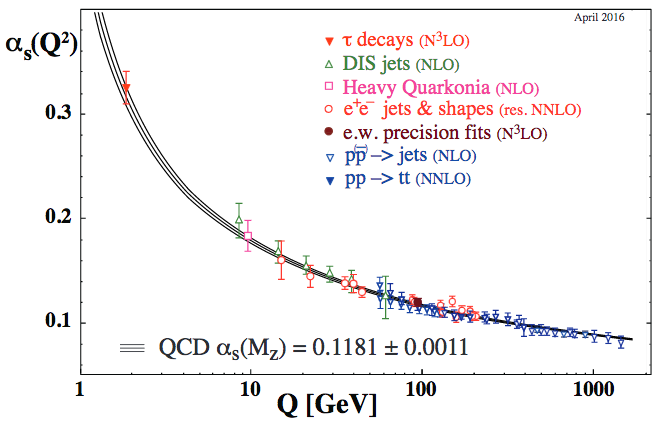
\includegraphics[width=0.95\textwidth]{figures/Chapter2/StrongCouplingConstant.png}
		\caption{Summary of measurements of $\alpha_{s}$ as a function of the energy scale $Q$. The respective degree of QCD perturbation theory used in the extraction of $\alpha_{s}$ is indicated in brackets (NLO: next-to-leading order; NNLO: next-to-next-to leading order; res. NNLO: NNLO matched with resummed next-to-leading logs; N\textsuperscript{3}LO: next-to-NNLO). Figure and caption taken from~\cite{Olive:2016xmw}.}
		\label{fig:strong_coupling_constant}
	\end{center}
\end{figure}

There are a few interesting facts about the strong interaction which must be noted.
In contrast to the electroweak interaction C, P, and T are all conserved.
Additionally, the strong force has a range of about $10^{-15}\unit{m}$, which is enough to act on nucleons, i.e. protons and neutrons, to form atomic nuclei.
Lastly, QCD is a strongly coupled theory at low energies and large distance scales and weakly interacting at high energies and small distance scales.
Quarks are confined particles, meaning that the attractive force between them does not decrease as they move farther apart.
Instead the force decreases as the particles move closer and increases as they move farther apart, a behavior called asymptotic freedom~\cite{PhysRevLett.30.1343}.
When in the high energy regime the typical perturbative calculation can be made, but in the low energy regime theorists must use more advanced techniques such as lattice gauge theory~\cite{Rothe2005}.

\section{Brout-Englert-Higgs Mechanism \& The Higgs Boson}
\label{sec:higgs_mechanism}

The EW and QCD Lagrangians covered in sections~\ref{sec:electroweak_interaction} and~\ref{sec:strong_interaction} contain no mass terms, which means the bosons within the SM should be massless.
However, we know from experiments at CERN that the $W^{\pm}$~\cite{ARNISON1983103} and $Z$~\cite{1983398} bosons do indeed have mass.
The method by which mass is added to the SM while maintaining the necessary gauge invariance is the BEH mechanism~\cite{PhysRevLett.13.321,PhysRevLett.13.508}.
This is accomplished by adding one or more complex scalar fields, the Higgs field(s), to the SM Lagrangian.
These fields will acquire a vacuum expectation value (vev) which will spontaneously break the symmetry of the Lagrangian.
The Goldstone theorem tells us that for every spontaneously broken continuous symmetry there will be a new massive scalar ``Goldstone'' boson.
So the number of Goldstone bosons will be equal to the number of broken generators of the symmetry group.
The massless standard model bosons then acquire mass by absorbing these Goldstone bosons.
So the number of massive SM bosons will be equal to the number of broken generators.

Remember from section~\ref{sec:electroweak_interaction} there are four massless electroweak gauge bosons, $W^{1}$, $W^{2}$, $W^{3}$, and $B^{0}$.
The experimentally observed bosons, however, are the massless photon ($\gamma$) and three massive bosons ($W^{\pm}$, $Z$).
We also know that the electric charge Q is conserved in electroweak interactions.
This means that the $SU\left(2\right)_{L}{\times}U\left(1\right)_{Y}$ electroweak theory is broken such that a new $U\left(1\right)_{EM}$ symmetry group is formed which corresponds to electromagnetism.
In order for three gauge bosons to acquire mass they must absorb three Goldstone bosons.
The simplest method to accomplish this is to introduce a complex, scalar $SU\left(2\right)$ doublet $\Phi$ with hypercharge $Y=1$.
\begin{equation}\label{eq:higgs_scalar_field}
	\Phi=\doublet[r]{\phi^{+}}{\phi^{0}}
\end{equation}
The part of the SM Lagrangian which includes the electroweak gauge bosons and the leptons can be written as
\begin{equation}
	\mathcal{L}_{SM}=-\frac{1}{4}W_{\mu\nu}^{a}W_{a}^{\mu\nu}-\frac{1}{4}B_{\mu\nu}B^{\mu\nu}+\bar{L}_{i}\left(iD_{\mu}\gamma^{\mu}\right)L_{i}+\bar{e}_{R,i}\left(iD_{\mu}\gamma^{\mu}\right)e_{R,i}
\end{equation}
where $i$ runs over the three generations, $\mu$ and $\nu$ are Lorentz indices, and $a$ runs over the generators in the gauge group.
The field strengths are given by
\begin{align}
	W_{\mu\nu}^{a}&=\partial_{\mu}W_{\nu}^{a}-\partial_{\nu}W_{\mu}^{a}+g_{2}\epsilon^{abc}W_{\mu}^{b}W_{\nu}^{c}\\
	B_{\mu\nu}&=\partial_{\mu}B_{\nu}-\partial_{\nu}B_{\mu}
\end{align}
and the covariant derivatives for the left- and right-handed leptons are
\begin{align}
	D_{\mu}L_{L}&=\left(\partial_{\mu}-ig_{2}T_{a}W_{\mu}^{a}-ig_{1}YB_{\mu}\right)L_{L}\\
	D_{\mu}e_{R}&=\left(\partial_{\mu}-ig_{1}YB_{\mu}\right)e_{R}
\end{align}
where $T_{a}$ are the generators of the $SU\left(2\right)_{}L$ gauge group and $g_{1}$, $g_{2}$ are the coupling constants for the electroweak interaction.

By adding the scalar field in equation~\ref{eq:higgs_scalar_field} we must add an additional scalar part to the Lagrangian
\begin{equation}
	\mathcal{L}_{Higgs}=\left(D^{\mu}\Phi\right)^{\dagger}\left(D_{\mu}\Phi\right)-V\left(\Phi\right)
\end{equation}
where the first term is the kinetic term and the second term is the scalar potential, also known as thr ``Mexican Hat'' potential.
While the form of the scalar potential is not known from first principles, we can make the assumption that it takes the simplest form possible which has the desired properties of spontaneous symmetry breaking and the ability to be renormalized
\begin{equation}
	V\left(\Phi\right)=\mu^{2}\Phi^{\dagger}\Phi+\lambda\left(\Phi^{\dagger}\Phi\right)^{2}
\end{equation}
The value of $\lambda$ must be positive in order for the vacuum to be stable.
The sign of $\mu^{2}$ specified one of two cases for the potential, both of which are illustrated in figure 

\begin{figure}[hbt]
	\begin{center}
		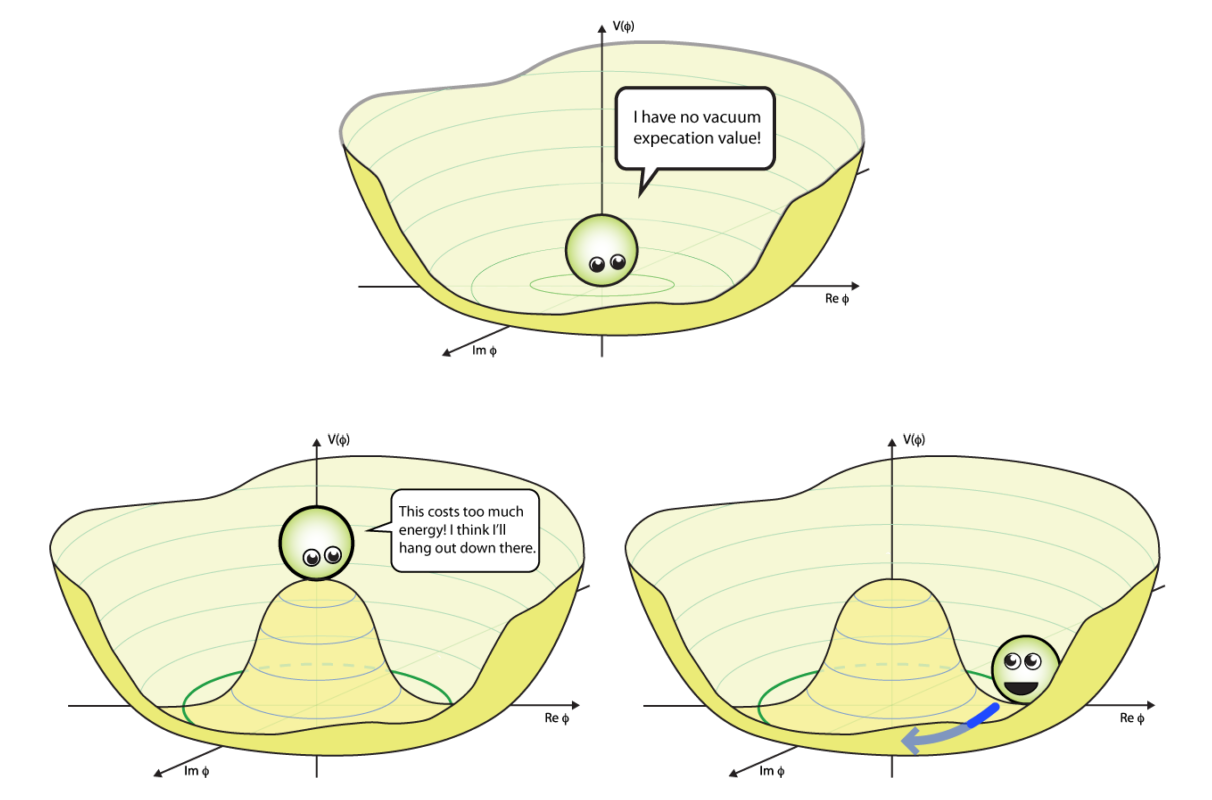
\includegraphics[width=0.95\textwidth]{figures/Chapter2/HiggsVEV.png}
		\caption{(Top) The scalar potential when $\mu^{2}>0$. In this case the potential will always be positive and its minimum value will be at the origin. The vacuum expectation value for this potential is zero. (Bottom) When $\mu^{2}<0$ the potential will take the shape of a ``Mexican Hat'' with its minimum value being in a degenerate ring around the origin. As soon as the scalar field has moves away from the origin and closer to the minimum the symmetry has been spontaneously broken and will acquire a non-zero vev. Because the scalar field picked a particular direction when falling towards the minimum, it is no longer invariant under a rotation~\cite{Tanedo}.}
		\label{fig:higgs_vev}
	\end{center}
\end{figure}






\begin{comment}
Higgs responsible for electroweak symmetry breaking (EWSB), discussed more in section~\ref{sec:higgs_mechanism}
	For electroweak interaction to be gauge invariant the gauge bosons corresponding to this force must be massless, which they aren't.
	Higgs mechanism solves this.
	Short version is that Higgs field causes a spontaneuous EWSB due to its non-zero vacuum expectation value (VEV)
	\begin{equation}
	\label{eq:spontaneous_symmetry_breaking}
	SU_{L}\left(2\right){\times}U_{Y}\left(1\right){\rightarrow}U_{EM}\left(1\right)
	\end{equation}
	allows fermion field to aquire mass, which it was forbidden to do from eqn.~\ref{eq:standard_model_groups}
	Higgs field contains a doublet of scalar bosons, two charged particles and two neutral particles.
		Two charged and one neutral combine with W$^{\pm}$ and Z to produce their masses
		Other neutral particle is the Higgs boson H
	Higgs boson 



SM Lagrangian density
\begin{equation}
\label{eq:SM_Lagrangian_density}
\ell_{SM}=\ell_{kinetic}+\ell_{Yukawa}+\ell_{Higgs}
\end{equation}
$\ell_{kinetic}$ = kintetic terms plus gauge interactions
\ell_{Yukawa} = contains terms coupling fermion fields to Higgs fields
\ell_{Higgs} = related to Higgs potential $V\left(\phi\right)$, through $\ell_{Higgs}=-V\left(\phi\right)$ where
\begin{equation}
\label{eq:Higgs_potential}
V\left(\phi\right)=-\mu^{2}|\phi^{\dagger}\phi|+\lambda\left(|\phi^{\dagger}\phi|\right)^{2}
\end{equation}
with $\mu^{2}>0$ and $\lambda>0$
Higgs potential minimized at non-zero value of Higgs field
	nonzero ground state or vacuum expectation value (vev)
	may be chosen so that real, enutral componenet is non-zero
	\begin{equation}
	\left<\phi\right>=\frac{1}{\sqrt{2}}\left(\begin{array}{c}0 \\\nu\end{array}\right)
	\end{equation}
	where $\nu^{2}=\frac{\mu^{2}}{\lambda}$
	vev is source of electroweak symmetry breaking.

If forces weak enough, can QFT calculations use perturbative method to calculate leading order (LO) term.
next-to-leading order (NLO) corretions added in, then next-to-next-to leading order (NNLO) and so on
\end{comment}




\begin{comment}
\begin{figure}[!hbt]
    \centering
    \begin{subfigure}[t]{0.48\textwidth}
        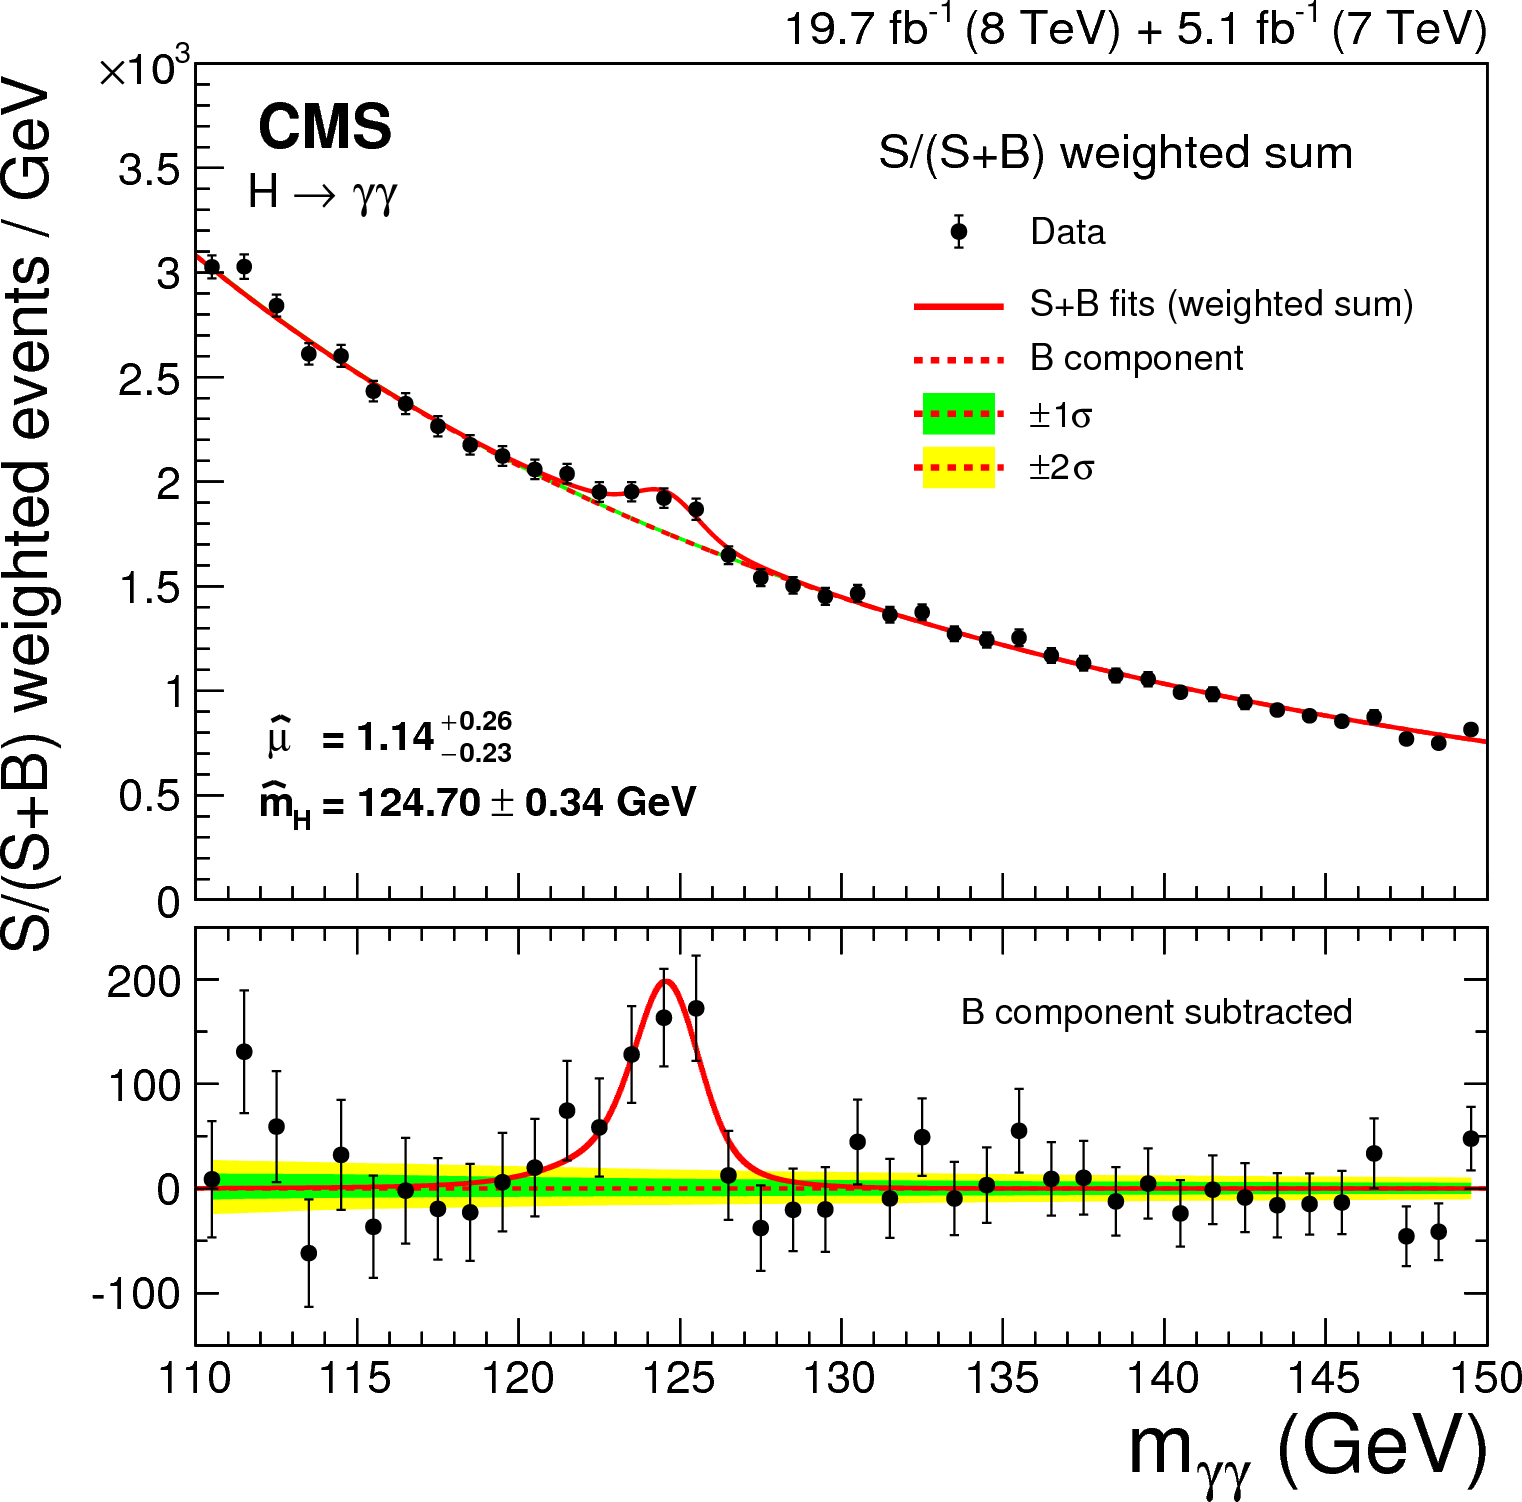
\includegraphics[width=\textwidth]{\figpath/Chapter2/HgammagammaPeak.png}
        \caption{}
        \label{fig:HgammagammaPeak}
    \end{subfigure}
    \begin{subfigure}[t]{0.48\textwidth}
        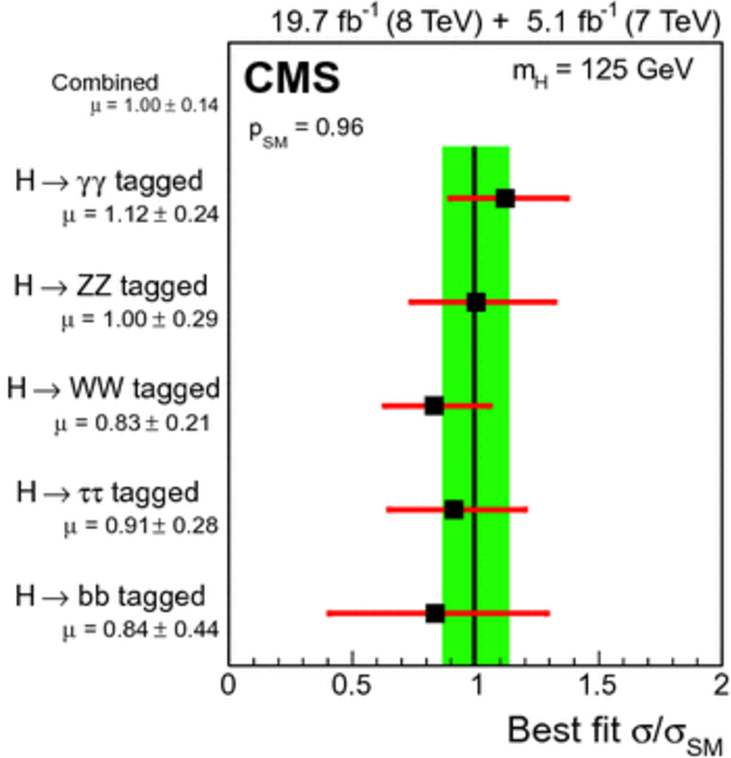
\includegraphics[width=\textwidth]{\figpath/Chapter2/10052_2015_3351_Fig4_HTML.pdf}
        \caption{}
        \label{fig:HiggsSignalStrength}
    \end{subfigure}
    \caption{(Left) The $H\rightarrow\gamma\gamma$ signal peak as seen in 2012~\cite{Hgammagamma}. (Right) Best-fit $\sigma/\sigma_{SM}$ grouped by predominant decay mode. The vertical band is the overall combined analysis value and the horizontal bars show the $\pm$1 uncertainties (statistical and systematic)~\cite{Khachatryan2015}.}
    \label{fig:HiggsIn2012}
\end{figure}
\end{comment}

%, as seen in figure~\ref{fig:Higgs_WW_lnujj_feynman}

%While at 125\gev the gluon-gluon fusion (ggF) production cross section\footnote{This analysis is independent of production mode, but selects for a specific decay channel.} and $l\nu{qq}$ branching ratio are high, as seen in figure~\ref{fig:Higgs_XS_and_BR}, there are significant experimental challenges to overcome.

\begin{comment}
\begin{figure}[bt]
	\centering
	\begin{subfigure}[t]{0.415\textwidth}
		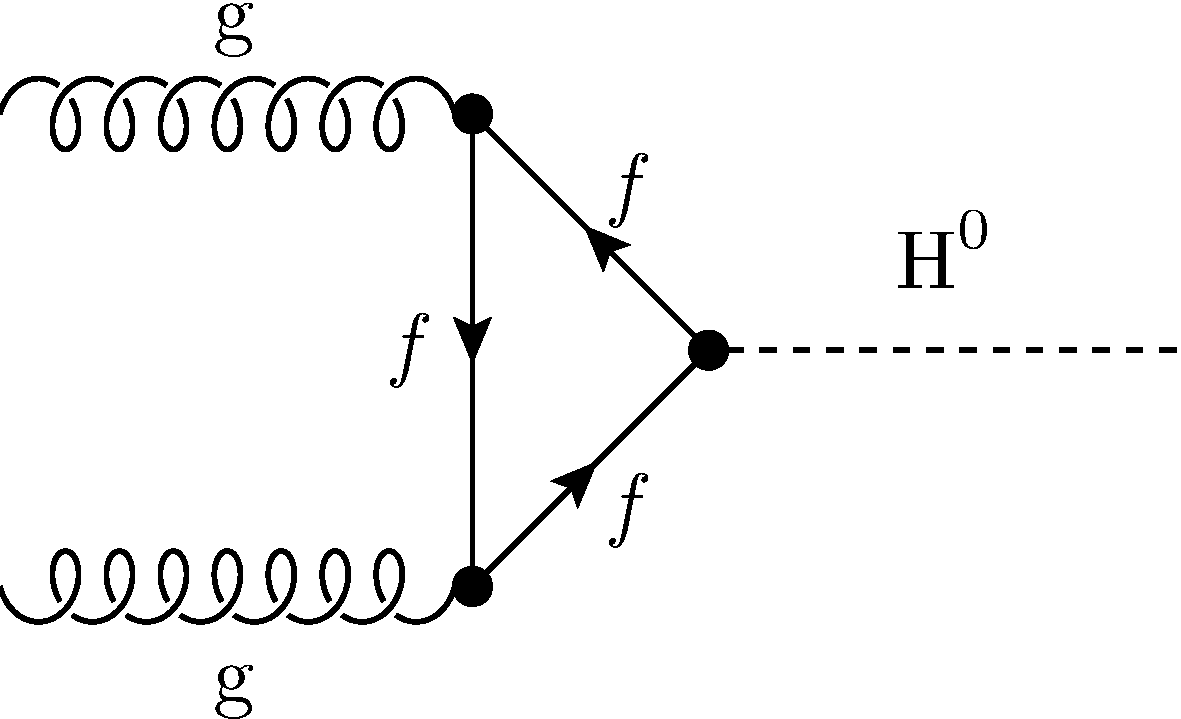
\includegraphics[width=\textwidth]{\figpath/FeynmanDiagrams/ggH.eps}
		\label{fig:ggH}
	\end{subfigure}%
	\begin{subfigure}[t]{0.415\textwidth}
		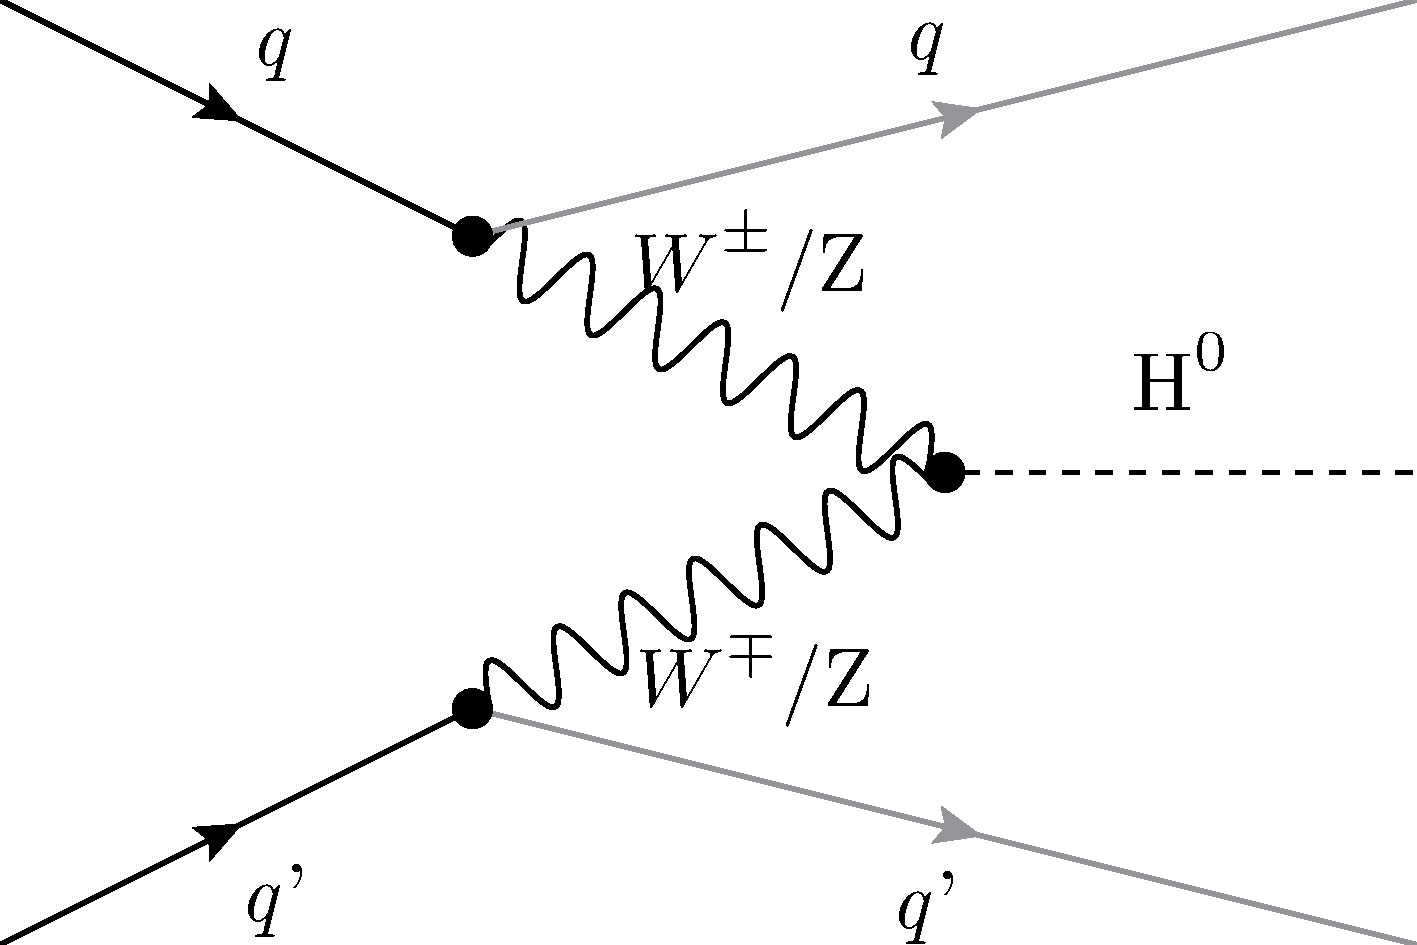
\includegraphics[width=\textwidth]{\figpath/FeynmanDiagrams/qqH.eps}
		\label{fig:qqH}
	\end{subfigure}

	\begin{subfigure}[t]{0.415\textwidth}
		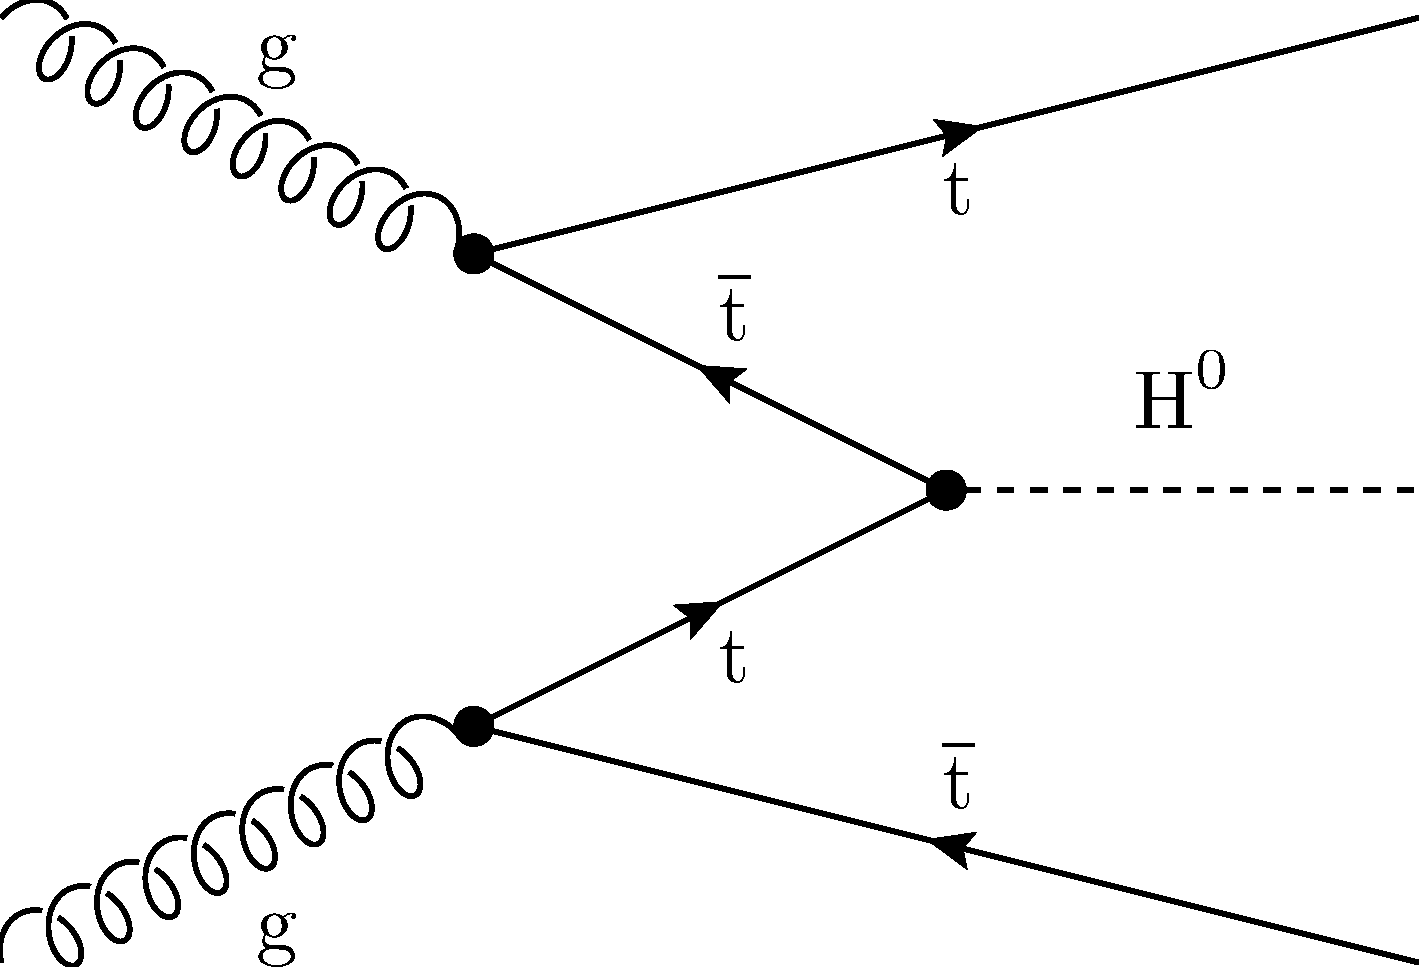
\includegraphics[width=\textwidth]{\figpath/FeynmanDiagrams/ttH.eps}
		\label{fig:ttH}
	\end{subfigure}%
	\begin{subfigure}[t]{0.415\textwidth}
		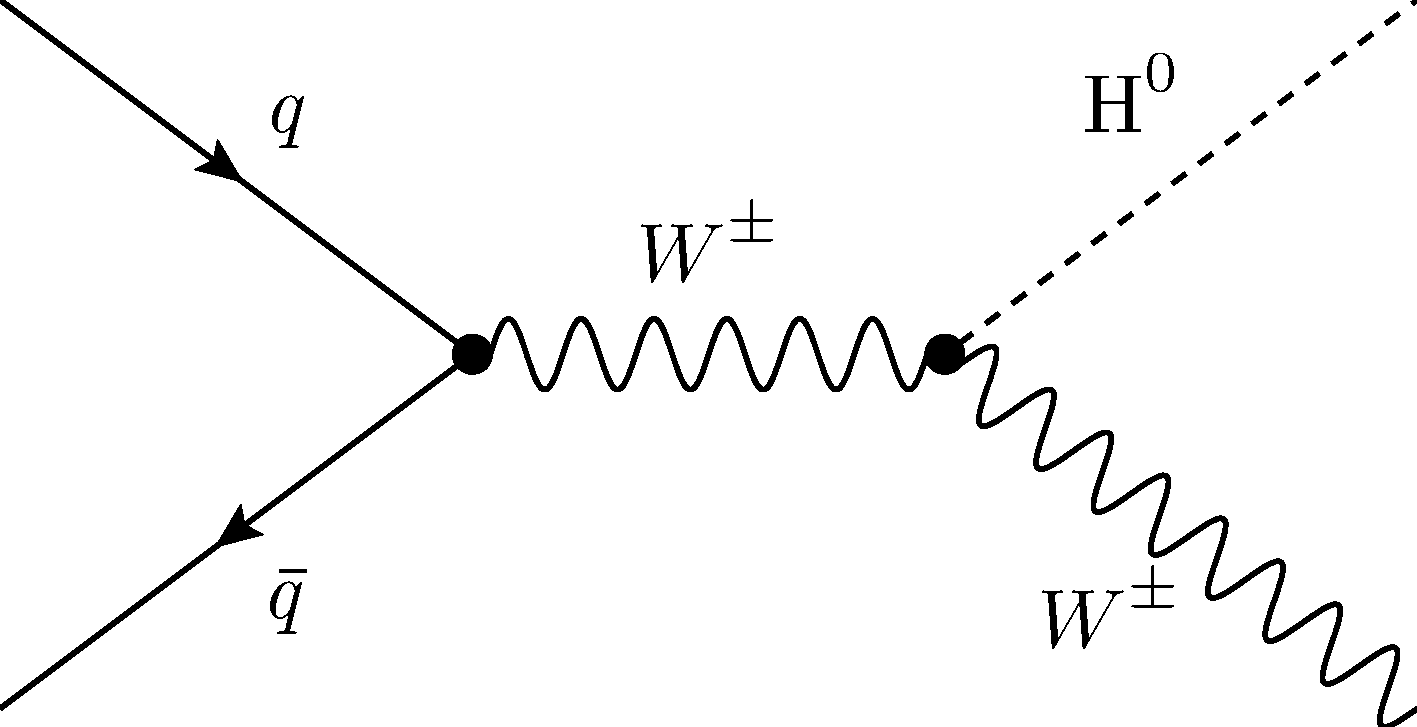
\includegraphics[width=\textwidth]{\figpath/FeynmanDiagrams/WH.eps}
		\label{fig:WH}
	\end{subfigure}
	\caption{Feynman diagrams for the four Higgs production mechanisms with associated $l{\nu}qq$ decays: gluon-gluon fusion (upper left), vector-boson fusion (upper right), \ttbar fusion (lower left), and associated production (lower right).}
	\label{fig:Higgs_WW_lnujj_feynman}
\end{figure}

\begin{figure}[!hbt]
	\centering
	\begin{subfigure}[t]{0.54\textwidth}
		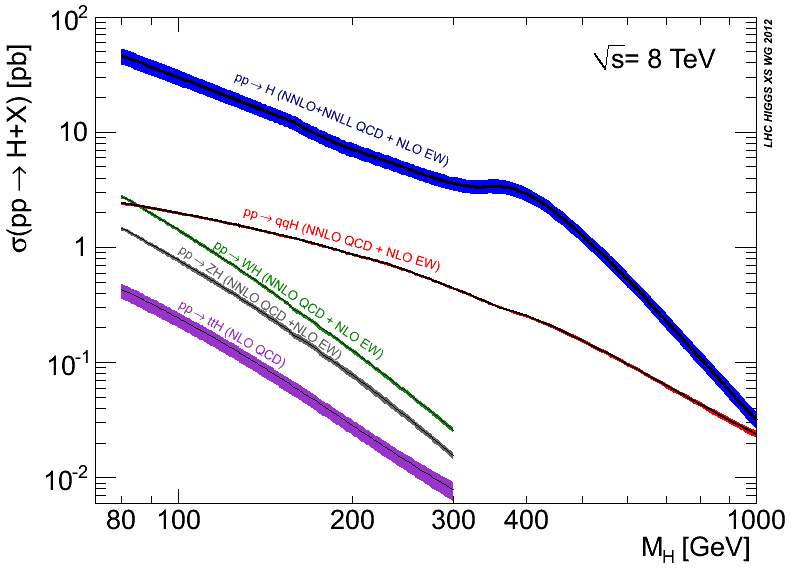
\includegraphics[width=\textwidth]{\figpath/Chapter2/Higgs_XS_8TeV.png}
		\label{fig:Higgs_XS_8TeV}
	\end{subfigure}
	\begin{subfigure}[t]{0.41\textwidth}
		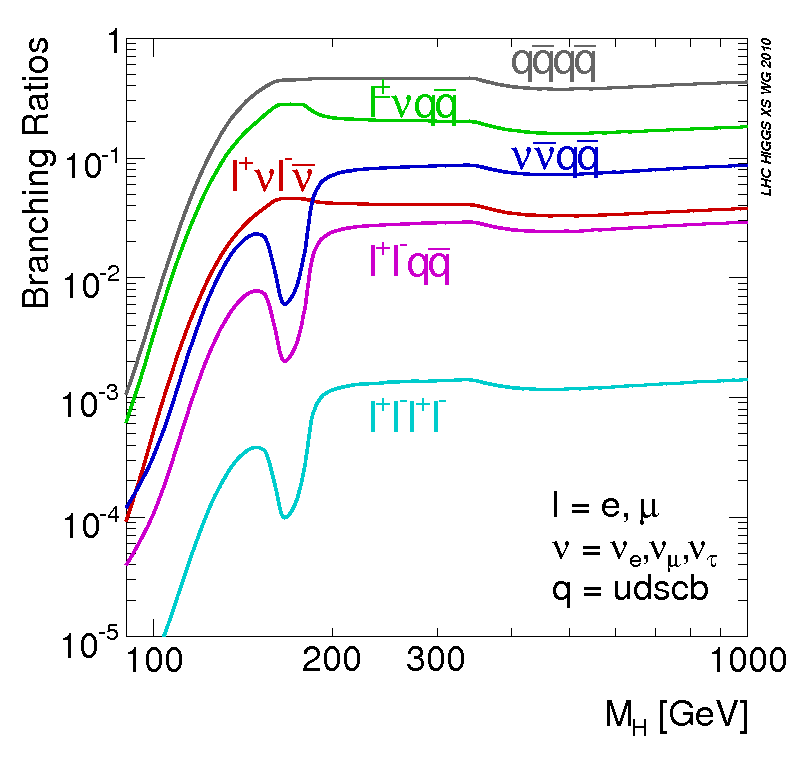
\includegraphics[width=\textwidth]{\figpath/Chapter2/Higgs_BR_4fermion.png}
		\label{fig:Higgs_BR_4fermion}
	\end{subfigure}
	\caption{The Standard Model Higgs production cross sections at 8\tev (left) and WW branching ratios to four fermion final states (right).}
	\label{fig:Higgs_XS_and_BR}
\end{figure}
\end{comment}

\begin{figure}[hbt]
	\begin{center}
		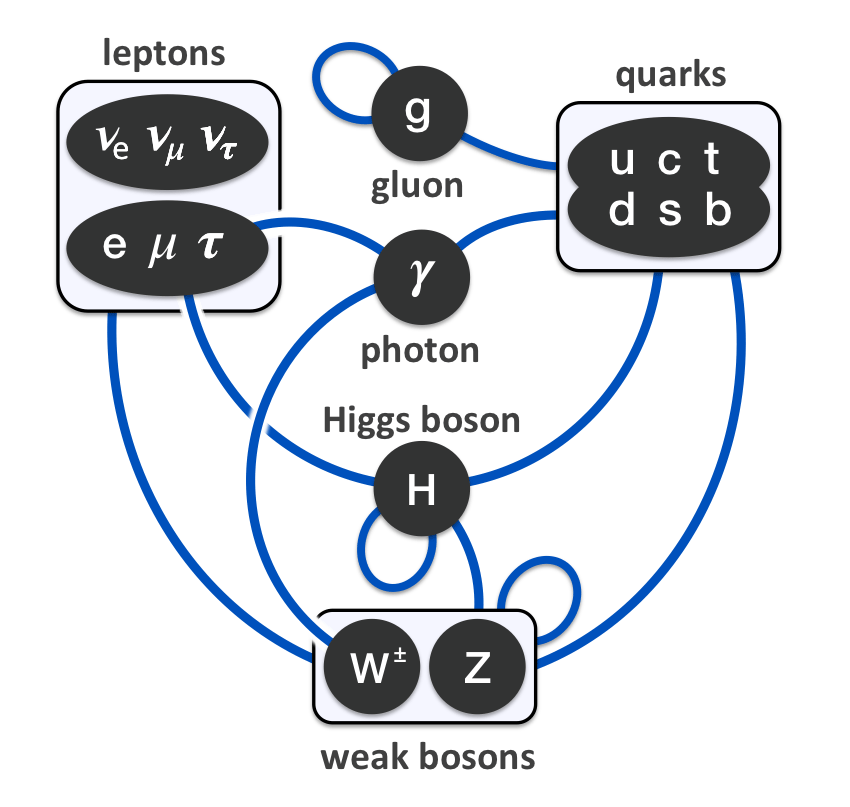
\includegraphics[width=0.95\textwidth]{figures/Chapter2/Elementary_particle_interactions_in_the_Standard_Model.png}
		\caption{A diagram illustrating the leading order interactions between particles in the standard model, including self-interactions~\cite{Drexler}.}
		\label{fig:sm-interactions}
	\end{center}
\end{figure}


\section{Beyond the Standard Model}
\label{sec:BSM}